 Inc.\documentclass[
  shortnames]{jss}

%% recommended packages
\usepackage{orcidlink,thumbpdf,lmodern}

\usepackage[utf8]{inputenc}

\author{
Gilberto Camara~\orcidlink{0000-0002-3681-487X}\\Nat Inst for Space Research\\
Brazil \And Renato Assunção~\orcidlink{0000-0001-7442-9166}\\ESRI Inc.\\
Brazil \And Rolf Simoes~\orcidlink{0000-0003-0953-4132}\\Nat Inst for Space Research\\
Brazil \AND Alexandre Carvalho~\orcidlink{0000-0001-8762-5465}\\Inst Applied Economic Research\\
Brazil \And Felipe Souza~\orcidlink{0000-XXXXX}\\Nat Inst for Space Research\\
Brazil \And Pedro R. Andrade~\orcidlink{0000-0001-8675-4046}\\Nat Inst for Space Research\\
Brazil
}
\title{Bayesian inference for smoothing of remote sensing image classification using machine learning}

\Plainauthor{Gilberto Camara, Renato Assunção, Rolf Simoes, Alexandre Carvalho, Felipe Souza, Pedro R. Andrade}
\Plaintitle{Bayesian smoothing for image classification}
\Shorttitle{Bayesian smoothing for image classification}


\Abstract{
The abstract of the article.
}

\Keywords{Bayesian smoothing, image classification, machine learning, \proglang{R}}
\Plainkeywords{Bayesian smoothing, image classification, machine learning, R}

%% publication information
%% \Volume{50}
%% \Issue{9}
%% \Month{June}
%% \Year{2012}
%% \Submitdate{}
%% \Acceptdate{2012-06-04}

\Address{
    Gilberto Camara\\
    Nat Inst for Space Research\\
Brazil\\
    Avenida dos Astronautas, 1758\\
12227-001 Sao Jose dos Campos, Brazil\\
  E-mail: \email{gilberto.camara```inpe.br}\\
  
            }


% tightlist command for lists without linebreak
\providecommand{\tightlist}{%
  \setlength{\itemsep}{0pt}\setlength{\parskip}{0pt}}

% From pandoc table feature
\usepackage{longtable,booktabs,array}
\usepackage{calc} % for calculating minipage widths
% Correct order of tables after \paragraph or \subparagraph
\usepackage{etoolbox}
\makeatletter
\patchcmd\longtable{\par}{\if@noskipsec\mbox{}\fi\par}{}{}
\makeatother
% Allow footnotes in longtable head/foot
\IfFileExists{footnotehyper.sty}{\usepackage{footnotehyper}}{\usepackage{footnote}}
\makesavenoteenv{longtable}



\usepackage{amsmath} \usepackage[english]{babel} \usepackage{microtype} \usepackage{graphicx} \usepackage{booktabs} \usepackage{float} \usepackage{flafter} \usepackage{placeins} \usepackage[all,defaultlines=3]{nowidow} \usepackage[T1]{fontenc} \usepackage[adobe-utopia]{mathdesign} \renewcommand*\ttdefault{txtt}

\begin{document}



\newpage

\hypertarget{introduction}{%
\section{Introduction}\label{introduction}}

Remote sensing images are crucial to environmental management. Its uses include measuring changes in land cover, agriculture, and natural habitats. Images identify and track wildfires, enabling timely response and effective response. Satellite measures are the only way to provide a systematic cover of large and distant areas; an example is detection of tropical deforestation, which is crucial in the fight against climate change. By providing vital information to policymakers and conservationists, remote sensing data helps protect the world's environment.

One of the most important tasks in remote sensing image processing is image classification, a task which partitions the pixels in an image into different classes based on their spectral characteristics, spatial patterns, or other relevant features. Machine learning methods such as random forests \citep{Belgiu2016} and deep learning \citep{Ma2019} are commonly used for this job. These techniques typically rely on training samples that are derived from single and isolated pixels, hand-picked by users to represent the desired output classes. The result of machine learning classification is usually a set of matrices with the same size as the original image. Each matrix contains the likelihoods for that a pixel belongs to one of the classes.

Post-processing techniques have become crucial to refine the labels of a classified image \citep{Huang2014}. There are a number of reasons why the post-processing is required. Classification algorithms may introduce noise or produce misclassifications due to the complexity of remote sensing data. At any resolution level, an image pixel only summarizeswhat is real. Pixels with mixed landscapes are common and this can misguide a classification technique. The pixel resolution is the size of the ground area that each pixel represents in the image. This ground area may not be homogeneously composed of a single class, especially on transition zones between different landscapes. The features associated with a given pixel are an amalgamation or fusion of the diverse elements on these mixed pixels and they may be hard to classify.

Another reason for post-processing is to refine the boundary between classes or to filter out outliers and misclassified pixels. The classification algorithms may produce noisy or fragmented class assignments, especially when dealing with high-resolution imagery. The features used to classify the pixels, such as their spectral characteristics, have large variability and different classes show great overlap. The consequence is that the classifiers often produce results with outliers or misclassified pixels. By mitigating these errors and minimizing noise, post-processing improves the quality of the initial classification results, bringing a significant gain in the overall accuracy and interpretability of the final output \citep{Schindler2012}.

Both reasons for post-processing are clearly seen in Figure \ref{fig:roim}, which shows a fragment of a Sentinel-2 image from the Amazon in the state of Rondonia, Brazil. The image starkly contrasts forest areas (depicted in green) and deforested areas (portrayed in various shades of orange and brown). However, we see the border pixels between different land classes with with less stark colors representing their fuzzy class assignment.

\begin{CodeChunk}
\begin{figure}[h]

{\centering 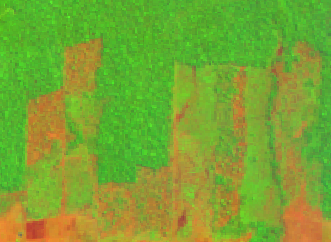
\includegraphics[width=4.6in]{images/rondonia_image} 

}

\caption[Sentinel-2 image of deforestation in the Amazon forest (detail)]{Sentinel-2 image of deforestation in the Amazon forest (detail).}\label{fig:roim}
\end{figure}
\end{CodeChunk}

Overall, post-processing of machine learning output in remote sensing image classification is essential to enhance the accuracy, spatial coherence, and interpretability of the classification results, ensuring that the final maps provide reliable information for decision-making and subsequent analysis. Most post-processing methods use the smoothness assumption that nearby pixels tend to have the same label \citep{Schindler2012}. These include probability-based smoothing methods such as Gaussian, semi-global, bilateral and edge-aware filtering \citep{Schindler2012}, modal filters \citep{Ghimire2010}, and co-occurrence matrices \citep{Huang2014}.

Despite their usefulness, these methods have shortcomings. Gaussian and semi-global smoothing assumes a single value of local variance per class for all neighborhoods. These methods also consider that pixel likelihoods change slowly within a neighborhood, and that the correlation depends only on how far two pixels are from each other \citep{Schindler2012}. Bilateral smoothing is an \textit{ad-hoc} method that introduces a global parameter that tries to preserve the shape of boundaries which are lost by Gaussian filters. The co-occurrence matrices proposed by \citet{Huang2014} work on categorical images and do not consider the likelihood values for each pixel. Also, these methods assume the spatial distribution of the class likelihoods is isotropic. When using the likelihood of a pixel and its neighbors to compute properties such as mean, variance and spatial autocorrelation, all spatial directions are considered equivalent. As we will argue in this paper, such assumption does not hold in general in the case of border pixels.

In this paper, we introduced a new type of post-processing algorithm founded on an Empirical Bayes approach and catered to the specific properties of land classification. The algorithm has been implemented in an R package, \pkg{bayesEO}. We employ non-isotropic neighbourhood definitions to mimic the effects of discontinuity between land classes, enabling our method to better capture the spatial complexities inherent in such data. Our method allows the inclusion of expert knowledge, removes outliers, and enhances the consistency of the resulting map. The \pkg{bayesEO} package can be used jointly with \pkg{sits}, an end-to-end toolkit for land use and land cover classification using big Earth observation data developed by the authors \citep{Simoes2021}.

Our package adds to the other \proglang{R} libraries focused on the spatial data analysis, including \pkg{spdep} \citep{Bivand2023} and \pkg{rgeoda} \citep{Li2022}. \pkg{CARBayes} \citep{Lee2013} implements Bayesian models for spatial areal units. For image processing analysis, \pkg{terra} \citep{Hijmans2023} provides supervised classification with decision trees, while \pkg{stars} \citep{Bivand2023} include functions for linear regression and random forest classification. For post-processing of machine learning image classification, \pkg{sits} also uses the method described in this paper. As far as we are aware, there is no current \proglang{R} package that supports post-processing of image classification of remote sensing images. Therefore, the \pkg{bayesEO} is a useful addition to the facilities available in \proglang{R} for remote sensing image processing.

\hypertarget{methods}{%
\subsection{Methods}\label{methods}}

In land classification, we deal with categorical data, with each category corresponding to a different land type (e.g., forest, grassland, water body). Land classification aims to subdivide the space into discrete areas, each associated with a distinct type of land use or cover. Borders between different land classes usually represent sharp transitions. Formally,
the land classification problem can be expressed as follows. Given a set of \(n\) spatial locations or pixels \(S = \{ \mathbf{s}_1, \ldots, \mathbf{s}_n \}\), each with an associated \(d\)-dimensional feature vector \(\mathbf{x}_1, \ldots, \mathbf{x}_s\) with values in \(\mathcal{X} \subset \mathbb{R}^m\).
and a set of \(m\) land classes \(K = \{ 1, ..., m \}\), we seek a classification function \(f\)
such that
\begin{align}
f\colon S \times \mathcal{X} \to K & \longrightarrow K \nonumber \\
(\mathbf{s}_i, \mathbf{x}_i) & \longmapsto (p_{i,1}, \ldots, p_{i,m}) 
\label{eq:classificationf}
\end{align}
with \(0 \leq p_{i,k} \leq 1\) and \(\sum_k p_{i,k} = 1 \forall i = 1, \ldots, n\).
The value \(p_{i,k}\) is interpreted as the probability that the \(i\)-th pixel belongs to the
\(k\)-th class. The class assigned to the pixel is determined by the highest probability among the available options. The left side of Figure \ref{fig:maps} shows such assignment produced by a random forest algorithm and explained in detail in section \textit{Software and examples}. However, this assignment can be problematic when the highest probability does not significantly surpass the others, resulting in an assignment with low confidence. This happens more frequently in pixels located at the transition zones between classes leading to noisy or fragmented class assignments.

\begin{CodeChunk}
\begin{figure}[h]

{\centering 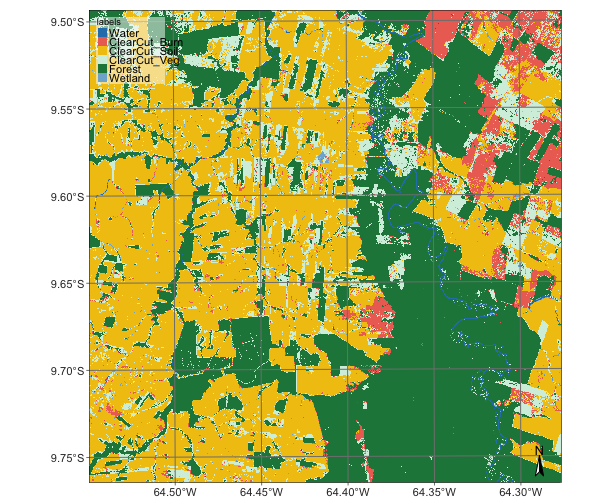
\includegraphics[width=0.49\linewidth,height=0.25\textheight]{images/map_no_smooth} 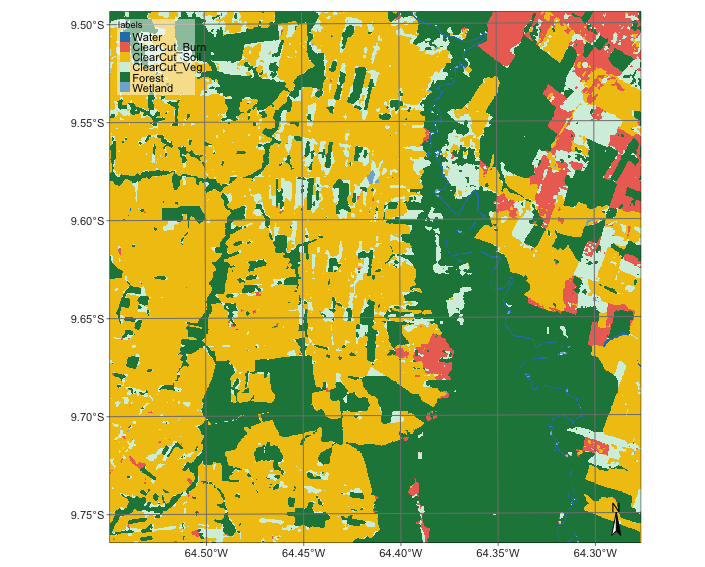
\includegraphics[width=0.49\linewidth,height=0.25\textheight]{images/map_smooth} 

}

\caption[Labelled maps without smoothing (left) and after smoothing (right) ]{Labelled maps without smoothing (left) and after smoothing (right) }\label{fig:maps}
\end{figure}
\end{CodeChunk}

Usually, the spatial \(\mathbf{s}_i\) is not explicitly used by the classification function \(f\). The reason is that \(f\) is obtained from a training dataset \(T = \{ \mathbf{s}_{t_1}, \ldots, \mathbf{s}_{t_s} \} \subset S\) with \(s \ll n\). Each element \(\mathbf{s}_{t_i} \in T\) is coupled with one single label \(k_{t_i} \in K\) representing the class to which it belongs, even when the pixel has mixed classes on the ground. This training dataset is also called the \textit{ground truth} dataset. Usually, it is composed of non-contiguous locations and therefore, there is no spatial neighborhood context available to train \(f\). The only resource to fit \(f\) are the true labels features \(\mathbf{x}\) measured at each location in the training dataset \(T\).

The main idea behind our post-processing method is that a pixel classification should take into account its neighborhood pixels. The right side of Figure \ref{fig:maps} shows the end result of applying our method on the random forest classification method shown in the left. We want to smooth the output and generate more coherent class representations, reducing the effects of small-scale variations or misclassifications. As the training dataset has no spatial context for the single pixels in \(T\), most remote sensing classification algorithms produce pixel-level classifications without considering the spatial coherence of neighboring pixels. This spatial coherence is introduced as a post-processing step.

\hypertarget{a-bayesian-approach}{%
\subsection{A Bayesian approach}\label{a-bayesian-approach}}

We initially consider a Bayesian approach for this task. Let \(\pi_{i,k} \geq 0\) be the prior probability of the \(i\)-th pixel belonging to class \(k \in \{1, \ldots, m\}\).
Converting probabilities to the logit scale allows for less modelling restrictions. Accordingly, let
\begin{equation*} 
\mu_{i,k} = \log\left( \frac{\pi_{i,k}}{1-\pi_{i,k}} \right) \sim N(m_{i,k}, s^2_{i,k}) 
\end{equation*}

The classification algorithm outputs the feature-based probabilities \((p_{i,1}, \ldots, p_{i,m})\) from (\ref{eq:classificationf}). We convert these observed values to the logit
scale and assumes a Gaussian distribution conditionally on \(\mu_{i,k}\):
\(x_{i,k} = \log(p_{i,k}/(1-p_{i,k})) \sim N(\mu_{i,k}, \sigma^2)\).
The variance \(\sigma^2_{k}\) will be estimated based on user expertise and taken as a hyperparameter to control the smoothness of the resulting estimate.

The standard Bayesian updating \citep{Gelman2014} leads to the posterior distribution
\begin{equation}
(\mu_{i,k} | x_{i,k}) \sim \sum N\left(  \frac{m_{i,t} \sigma^2_{k} +
    x_{i,k} s^2_{i,k}}{ \sigma^2_{k} +s^2_{i,k}} , \left( \frac{1}{\sigma_k^2} + \frac{1}{s^2_{i,k}} \right)^{-1} \right) 
\label{eq:BayesUpdate}
\end{equation}

The posterior mean, expressed as a weighted average between the pixel value \(x_{i,k}\)
and the prior mean \(m_{i,k}\), plays a crucial role. When the prior variance \(s^2_{i,k}\)
is high, the algorithm assigns more weight to the pixel value \(x_{i,k}\). Conversely, as the likelihood variance \(\sigma^2_k\) increases, the method assigns more weight to the prior mean
\(m_{i,k}\).

There are three aspects that must be taken into account to proceed. First, there is usually
no prior information to specify \(m_{i,k}\) and \(s^2_{i,k}\). Because of that, we will adopt an Empirical Bayes (EB) approach to obtain estimates of these prior parameters. Second, this method is not considering the pixel neighborhood. To deal with this, we will apply the EB
locally in a neighborhood of each pixel.

The third aspect is the most relevant one. A plain neighborhood of each pixel, based uniquely on the distance between locations, did not produce reasonable results. We must consider non-isotropic neighborhoods \(\mathcal{N}_{i,k}\) specific for each class \(k\) and pixel \(i\). The reason is that we want to give more weight to those neighborhood pixels with assignment classes with large probabilities as those are the ones estimated more reliably by the classification algorithm. We use an \(L\)-statistic to estimate \(m_{i,k}\) and \(s^2_{i,k}\) in our EB approach.
Let \(\alpha \in (0, 1)\) and \(W_{i}\) be the set of \(w\) nearest neighbors of pixel \(i\) (excluding the \(i\)-th pixel itself).
Also, let \(\mathbb{F}_{i,k}\) be the empirical distribution of the \(x_{j,k}\) for \(j \in W_i\).
Then, we take
\begin{equation}
\hat{m}_{i,k} = \frac{1}{1-\alpha} \int_{\alpha}^{\infty} \mathbb{F}_{i,k}^{-1}(s) ~ ds \: , 
\end{equation}
the average of the largest \((1-\alpha)\)-th fraction order statistics of the \(p_{i,k}\) logit transformed observations. Likewise, based on the these same \((1-\alpha)\)-th subset,
we obtain an empirical estimate \(\hat{s}^2_{i,k}\). The values of \(\hat{m}_{i,k}\) and\\
\(\hat{s}^2_{i,k}\) are used in the Bayesian updating (\ref{eq:BayesUpdate}).

\hypertarget{effect-of-the-hyperparameter}{%
\subsection{Effect of the hyperparameter}\label{effect-of-the-hyperparameter}}

The parameter \(\sigma^2_k\) controls the level of smoothness. If \(\sigma^2_k\) is zero, the estimated value \({E}[\mu_{i,k} | x_{i,k}]\) will be the pixel value \(x_{i,k}\). Values of the likelihood variance \(\sigma^2_{k}\), which are small relative to the prior variance \(s^2_{i,k}\) increase our confidence in the original probabilities. Conversely, likelihood variances \(\sigma^2_{k}\), which are large relative to the prior variance \(s^2_{i,k}\), increase our confidence in the average probability of the neighborhood.

Thus, the parameter \(\sigma^2_{k}\) expresses confidence in the inherent variability of the distribution of values of a class \(k\). The smaller the parameter \(\sigma^2_{k}\), the more we trust the estimated probability values produced by the classifier for class \(k\).
Conversely, higher values of \(\sigma^2_{k}\) indicate lower confidence in the classifier outputs and improved confidence in the local average values.

Consider the following two-class example. Take a pixel \(i\) with probability \(0.4\) (logit \(x_{i,1} = -0.4054\)) for class A, and probability \(0.6\) (logit \(x_{i,2} = 0.4054\)) for class B. Without post-processing, the pixel will be labelled as class B. Consider a local average of \(0.6\) (logit \(m_{i,1} = 0.4054\)) for class A and \(0.4\) (logit \(m_{i,2} = -0.4054\)) for class B. This is an outlier classified as class B in the midst of a set of pixels of class A.

Given this situation, we apply the proposed method. Suppose the local variance of logits to be \(s^2_{i,1} = 5\) for class A and \(s^2_{i,2} = 10\) and for class B. This difference is to be expected if the local variability of class A is smaller than that of class B. To complete the estimate, we need to set the parameter \(\sigma^2_{k}\), representing our belief in the variability of the probability values for each class.

Setting \(\sigma^2_{k}\) will be based on our confidence in the local variability of each class around pixel \({i}\). If we considered the local variability to be high, we can take both \(\sigma^2_1\) for class A and \(\sigma^2_2\) for class B to be both 10. In this case, the Bayesian estimated probability for class A is \(0.52\) and for class B is \(0.48\) and the pixel will be relabelled as being class A.

By contrast, if we consider local variability to be high If we set \(\sigma^2\) to be 5 for both classes A and B, the Bayesian probability estimate will be \(0.48\) for class A and \(0.52\) for class B. In this case, the original class will be kept. Therefore, the result is sensitive to the subjective choice of the hyperparameter.

\newpage

\hypertarget{defining-non-isotropic-neighbourhoods}{%
\subsection{Defining non-isotropic neighbourhoods}\label{defining-non-isotropic-neighbourhoods}}

The fundamental idea behind Bayesian smoothing for land classification posits that image patches with similar characteristics usually have a dominant class. This dominant class is marked by higher average probabilities and lower variance compared to other classes. In such regions, a pixel assigned to a different class is likely to exhibit lower average probabilities and higher local variance. As a result, post-processing should adjust the class of this pixel to match the dominant class.

Classification challenges arise for pixels located along the boundaries between areas containing different classes, as they possess signatures of two classes. In these cases, only some of the neighbours of such boundary pixels belong to the same class. To address this issue, we employ a non-isotropic definition of a neighbourhood to estimate the prior class distribution.

The non-isotropic neighborhood definition is selected as a subset of the logits of all values in a user-defined window. For instance, consider a boundary pixel with a neighborhood defined by a 7 x 7 window, located along the border between the \code{Forest} and \code{Grassland} classes. To estimate the prior probability of the pixel being a \code{Forest}, we should only take into account the neighbours on one side of the border that are likely to be correctly classified as \code{Forest}. Pixels on the opposite side of the border should be disregarded, since they are unlikely to belong to the same spatial process. In practice, we use only half of the pixels in the 7 x 7 window, opting for those that have a higher probability of being \code{Forest}. For the prior probability of the \code{Grassland} class, we reverse the selection and only consider those on the opposite side of the border.

Although this choice of neighbourhood may seem unconventional, it is consistent with the assumption of non-continuity of the spatial processes describing each class. A dense forest patch, for example, will have pixels with strong spatial autocorrelation for values of the \code{Forest} class; however, this spatial autocorrelation doesn't extend across its border with other land classes.

\hypertarget{software-and-examples}{%
\section{Software and examples}\label{software-and-examples}}

\hypertarget{reading-a-probability-data-cube}{%
\subsection{Reading a probability data cube}\label{reading-a-probability-data-cube}}

The input for post-classification is an image with probabilities produced by a machine learning algorithm. This file should be multi-band, where each band contains the pixel probabilities of a single class. The file name must have information on reference dates and include a version number. In the examples, we use a file produced by a random forest algorithm applied to a data cube of Sentinel-2 images for tile ``20LLQ'' in the period 2020-06-04 to 2021-08-26. The image has been stored as INT2S data type with integer values between {[}0..10000{]} to represent probabilities ranging from 0 ro 1.

\begin{CodeChunk}
\begin{CodeInput}
R> data_dir <- system.file("/extdata/Rondonia-20LLQ/", package = "sitsdata")
R> probs_file <- list.files(data_dir)
R> probs_file
\end{CodeInput}
\begin{CodeOutput}
[1] "SENTINEL-2_MSI_20LLQ_2020-06-04_2021-08-26_probs_v1.tif"
\end{CodeOutput}
\end{CodeChunk}

The training data has six classes: (a) \code{Forest} for natural tropical forest; (b) \code{Water} for lakes and rivers; (c) \code{Wetlands} for areas where water covers the soil in the wet season; (d) \code{ClearCut_Burn} for areas where fires cleared the land after tree removal. (e) \code{ClearCut_Soil} where the forest has been removed; (f) \code{ClearCut_Veg} where some vegetation remains after most trees have been removed. The class labels should also be informed by the user, since they are not stored in image files.

\begin{CodeChunk}
\begin{CodeInput}
R> labels <- c("Water", "ClearCut_Burn", "ClearCut_Soil",
+             "ClearCut_Veg", "Forest", "Wetland")
\end{CodeInput}
\end{CodeChunk}

The following code reads the file using the \code{terra} package.

\begin{CodeChunk}
\begin{CodeInput}
R> probs_image <- terra::rast(paste0(data_dir,"/",probs_file))
R> names(probs_image) <- labels
\end{CodeInput}
\end{CodeChunk}

The output is a \code{SpatRaster} object from the \code{terra} package. Figure \ref{fig:pcube} shows the plot of all layers of the probability image. The map for class \code{Forest} shows high probability values associated with compact patches and linear stretches in riparian areas. Class \code{ClearCut_Soil} is mostly composed of dense areas of high probability whose geometrical boundaries result from forest cuts. By contrast, the probability maps for classes \code{Water}, \code{ClearCut_Burn}, and \code{ClearCut_Veg} have mostly low values. Note that we need to inform the scaling parameter that converts the image to {[}0..1{]} interval.

\begin{CodeChunk}
\begin{CodeInput}
R> bayes_plot(probs_image, scale = 0.0001)
\end{CodeInput}
\begin{figure}[h]

{\centering 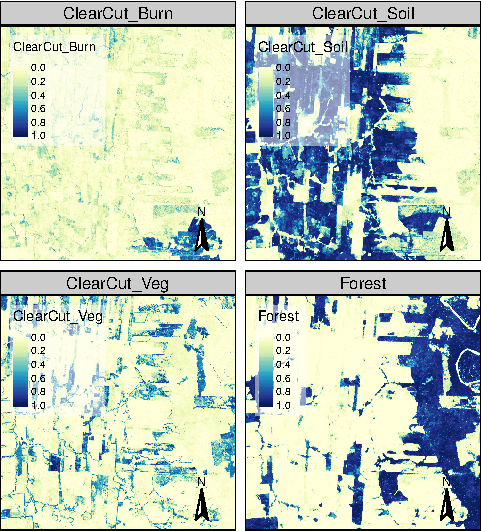
\includegraphics{Bayesian_smoothing_JSS_files/figure-latex/pcube-1} 

}

\caption[Class probabilities produced by random forest algorithm]{Class probabilities produced by random forest algorithm.}\label{fig:pcube}
\end{figure}
\end{CodeChunk}

Figure \ref{fig:map1} shows the resulting map, obtained by taking the class of higher probability to each pixel, without considering the spatial context. The non-smoothed labelled map shows the need for post-processing, since it contains a significant number of outliers and misclassified pixels. The map is produced by \code{bayes_label()} whose parameter is a \code{SpatRaster} object containing the probabilities of each class for all pixels. Then the map is rendered using \code{bayes_map()}.

\begin{CodeChunk}
\begin{CodeInput}
R> map_no_smooth <- bayes_label(probs_image)
\end{CodeInput}
\end{CodeChunk}

\begin{CodeChunk}
\begin{CodeInput}
R> bayes_map(map_no_smooth)
\end{CodeInput}
\begin{figure}[h]

{\centering 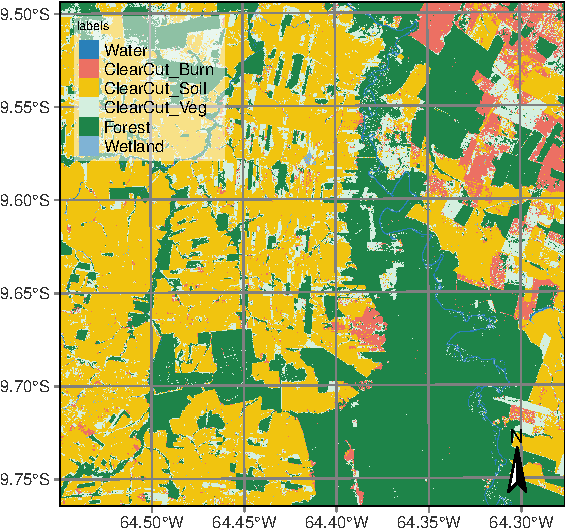
\includegraphics{Bayesian_smoothing_JSS_files/figure-latex/map1-1} 

}

\caption[Labelled map without smoothing]{Labelled map without smoothing.}\label{fig:map1}
\end{figure}
\end{CodeChunk}

\newpage

\hypertarget{estimating-the-local-logit-variances}{%
\subsection{Estimating the local logit variances}\label{estimating-the-local-logit-variances}}

The local logit variances correspond to the \(s^2_{i,k}\) parameter in the Bayesian inference and are estimated by \code{sits_variance()}. Its main parameters are: (a) a \code{SpatRaster} object ; (b) \code{window_size}, dimension of the local neighbourhood; (c) \code{neigh_fraction}, the percentage of pixels in the neighbourhood used to calculate the variance. The example below uses half of the pixels of a \(7\times 7\) window to estimate the variance. The chosen pixels will be those with the highest probability pixels to be more representative of the actual class distribution. The output values are the logit variances in the vicinity of each pixel.

\begin{CodeChunk}
\begin{CodeInput}
R> var_image <- bayes_variance(
+     x = probs_image,
+     window_size = 7)
R> bayes_summary(var_image)
\end{CodeInput}
\begin{CodeOutput}
 Water             ClearCut_Burn       ClearCut_Soil      ClearCut_Veg      
 Min.   : 0.0000   Min.   : 0.001214   Min.   : 0.00000   Min.   : 0.00000  
 1st Qu.: 0.1612   1st Qu.: 0.068792   1st Qu.: 0.09474   1st Qu.: 0.09772  
 Median : 2.0534   Median : 0.159645   Median : 0.23852   Median : 0.24155  
 Mean   : 2.4927   Mean   : 0.440458   Mean   : 0.84096   Mean   : 0.68647  
 3rd Qu.: 4.6397   3rd Qu.: 0.350913   3rd Qu.: 0.64510   3rd Qu.: 0.71808  
 Max.   :22.2649   Max.   :11.051078   Max.   :10.59077   Max.   :19.33537  
 Forest            Wetland           
 Min.   : 0.0000   Min.   : 0.00000  
 1st Qu.: 0.1026   1st Qu.: 0.07217  
 Median : 0.4152   Median : 0.17997  
 Mean   : 1.5687   Mean   : 0.71777  
 3rd Qu.: 2.2834   3rd Qu.: 0.42095  
 Max.   :25.7454   Max.   :10.66211  
\end{CodeOutput}
\end{CodeChunk}

The choice of the \(7 \times 7\) window size is a compromise between having enough values to
estimate the parameters of a normal distribution and the need to capture local effects
for class patches of small sizes. Classes such as \code{Water} and \code{ClearCut_Burn}
tend to be spatially limited; a bigger window size could result in invalid values for
their respective normal distributions.

The summary statistics show that most local variance values are low, which is an expected result. Areas of low variance correspond to pixel neighborhoods of high logit values for one of the classes and low logit values for the others. High values of the local variances are relevant in areas of confusion between classes. Figure \ref{fig:vcube} shows the values of local logit variances for classes \code{ClearCut_Soil} and \code{Forest}, considering only the \(4^{th}\) quartile of the distribution. Only the top 25\% of the values for each class are shown, emphasizing areas of high local variability.

\begin{CodeChunk}
\begin{CodeInput}
R> bayes_plot(var_image, quantile = 0.75, labels = c("ClearCut_Soil", "Forest"))
\end{CodeInput}
\begin{figure}[h]

{\centering 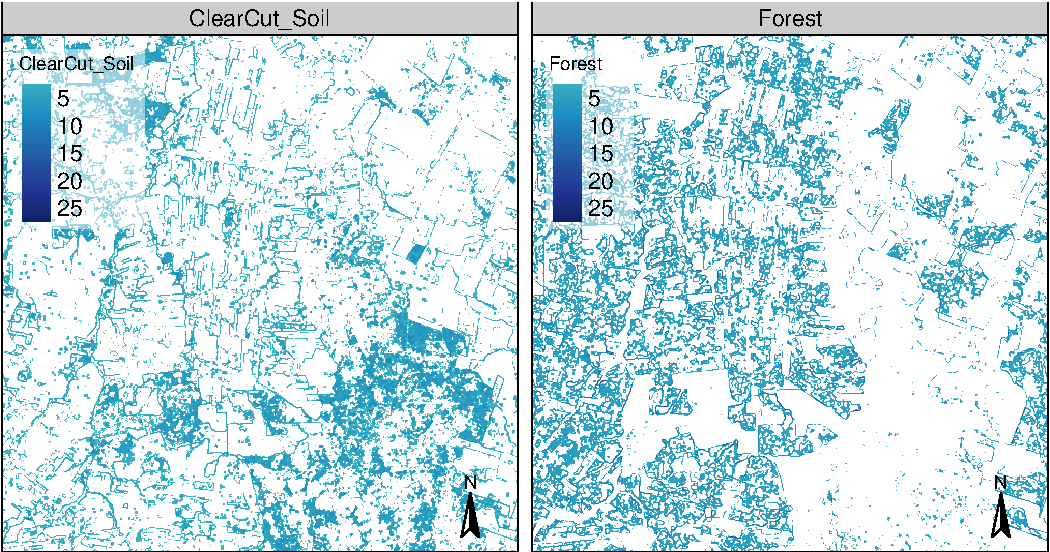
\includegraphics{Bayesian_smoothing_JSS_files/figure-latex/vcube-1} 

}

\caption[Logit variance map showing values above the 3rd quartile]{Logit variance map showing values above the 3rd quartile.}\label{fig:vcube}
\end{figure}
\end{CodeChunk}

Comparing the logit variance maps of Figure \ref{fig:vcube} with the probability maps of Figure \ref{fig:pcube} emphasizes the relevance of expert knowledge. The areas of high probability of class \code{Forest} are mostly made of compact patches; areas of high local variance occur near the borders of these patches. By contrast, class \code{ClearCut_Veg} represents a transition between natural forest areas and places where all trees have been cut, which are associated to class \code{ClearCut_Soil}. Class \code{ClearCut_Veg} has a high spectral variability, since the extent of remaining vegetation after most trees have been removed is not uniform. For this reason, the local variance of class \code{ClearCut_Veg} is mostly patch-based, while that of class \code{Forest} is mostly border-based.

Further insights are provided by Figure \ref{fig:vhist}, which shows the histograms of local variances per class. The values shown correspond to the \(4^{th}\) quartile (top 25\% of all values). The distribution of logit variances is uneven between the classes. Class \code{ClearCut_Veg} has a more balanced distribution, while most values in the \(4^{th}\) quartile of class \code{ClearCut_Soil} have low values.

\begin{CodeChunk}
\begin{CodeInput}
R> bayes_hist(var_image, quantile = 0.75)
\end{CodeInput}
\begin{figure}[h]

{\centering 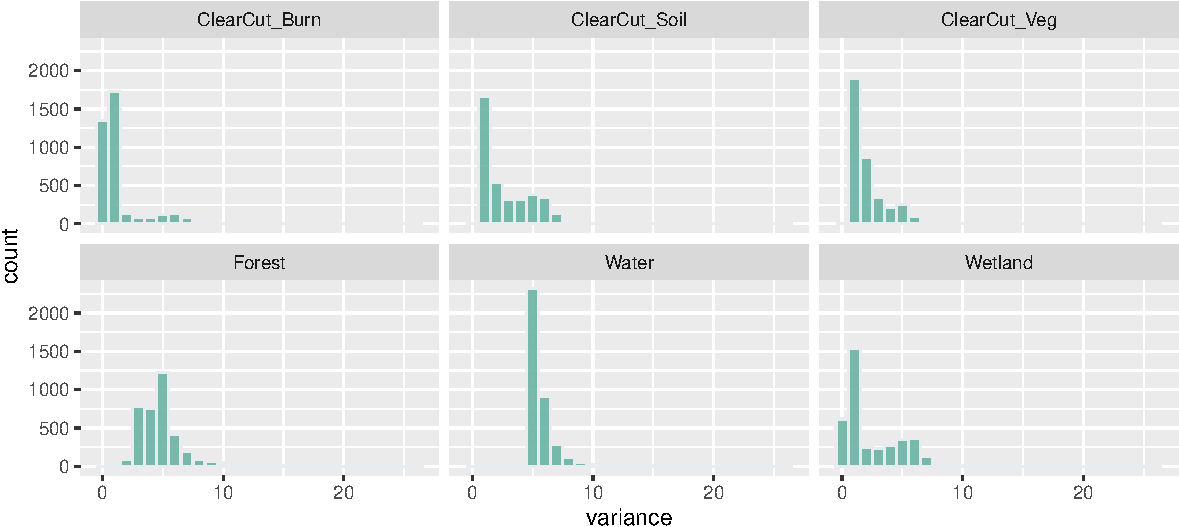
\includegraphics{Bayesian_smoothing_JSS_files/figure-latex/vhist-1} 

}

\caption[Histogram of top quartile of variances of class logits]{Histogram of top quartile of variances of class logits.}\label{fig:vhist}
\end{figure}
\end{CodeChunk}

\hypertarget{applying-bayesian-smoothing-to-remove-outliers}{%
\subsection{Applying Bayesian smoothing to remove outliers}\label{applying-bayesian-smoothing-to-remove-outliers}}

As discussed above, the effect of the Bayesian estimator depends on the values of the a priori variance \(\sigma^2_{k}\) set by the user and the neighbourhood definition to compute the local variance \(s^2_{i,1}\) for each pixel. To show the effects of different \(\sigma^2\) values we consider two cases: (a) setting \(\sigma^2\) to a high value close to the maximum value of local logit variance; (b) setting \(\sigma^2\) to a lower value close to the minimum value of the \(4^{th}\) quartile. To remove the outliers in the classification map, \pkg{bayesEO} provides \code{bayes_smooth()}. Its main parameters are: (a) \code{x}, a probability image; (b) \code{window_size}, dimension of the local neighbourhood; (c) \code{smoothness}, prior logit variances for each class. We first consider the case of high \(\sigma^2\) values.

\begin{CodeChunk}
\begin{CodeInput}
R> smooth_high <- bayes_smooth(
+     probs_image,
+     window_size = 7,
+     smoothness = c(25, 10, 20, 20, 25, 10)
+ )
\end{CodeInput}
\end{CodeChunk}

The impact of Bayesian smoothing can be best captured by producing a labelled map using \code{bayes_label()}, taking the smoothed image as its input. Figure \ref{fig:smth1} shows that the outliers and isolated pixels have been removed.

\begin{CodeChunk}
\begin{CodeInput}
R> map_smooth_high <- bayes_label(smooth_high)
R> bayes_map(map_smooth_high)
\end{CodeInput}
\begin{figure}[h]

{\centering 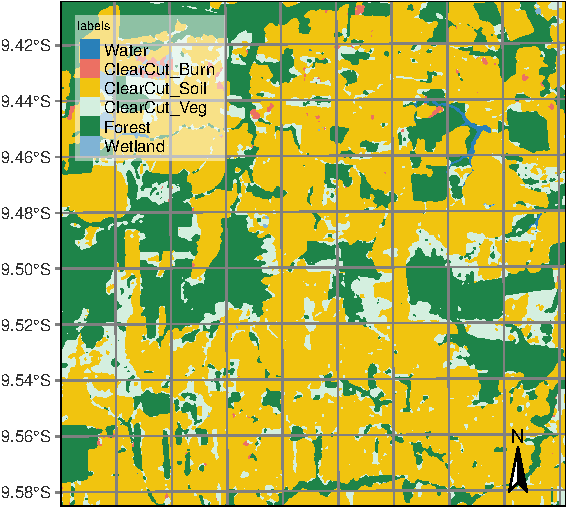
\includegraphics{Bayesian_smoothing_JSS_files/figure-latex/smth1-1} 

}

\caption[Labeled map with smoothing with high smoothness values]{Labeled map with smoothing with high smoothness values.}\label{fig:smth1}
\end{figure}
\end{CodeChunk}

In the smoothed map, the outliers have been removed by expanding \code{Forest} areas. Forests have replaced small corridors of water and soil encircled by trees. This effect is due to the high probability of forest detection in the training data. Compare the smoothing with high values with the smoothing with values close to the minimum value of the \(4^{th}\) quartile of the local variance for each class, as computed below.

\begin{CodeChunk}
\begin{CodeInput}
R> smooth_low <- bayes_smooth(
+     probs_image,
+     window_size = 7,
+     smoothness = c(5, 1, 1, 2, 4, 1)
+ )
\end{CodeInput}
\end{CodeChunk}

To see the impact of small \(\sigma^2\), we compute the labeled map.

\begin{CodeChunk}
\begin{CodeInput}
R> map_smooth_low <- bayes_label(smooth_low)
R> bayes_map(map_smooth_low)
\end{CodeInput}
\begin{figure}[h]

{\centering 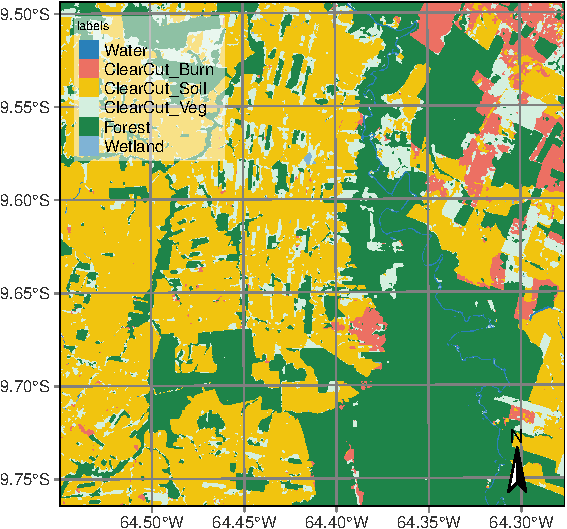
\includegraphics{Bayesian_smoothing_JSS_files/figure-latex/smth2-1} 

}

\caption[Labeled map with low smoothing parameters]{Labeled map with low smoothing parameters.}\label{fig:smth2}
\end{figure}
\end{CodeChunk}

A visual comparison between the two smoothed maps shows that there is an increase in the area of the \code{ClearCut_Veg} class. Such observation is confirmed by comparing the class areas of the non-smoothed map with the two types of smoothed maps, as shown below.

\begin{CodeChunk}
\begin{CodeInput}
R> sum1 <- bayes_summary(map_no_smooth)
R> colnames(sum1) <- c("class", "area_k2_no_smooth")
R> sum2 <- bayes_summary(map_smooth_high)
R> colnames(sum2) <- c("class", "area_k2_smooth_high")
R> sum3 <- bayes_summary(map_smooth_low)
R> colnames(sum3) <- c("class", "area_k2_smooth_low")
R> dplyr::inner_join(sum1, sum2, by = "class") |>  
+   dplyr::inner_join(sum3, by = "class")
\end{CodeInput}
\begin{CodeOutput}
# A tibble: 6 x 4
  class         area_k2_no_smooth area_k2_smooth_high area_k2_smooth_low
  <chr>                     <dbl>               <dbl>              <dbl>
1 Water                      6.26                4.15               4.72
2 ClearCut_Burn             52.6                43.2               44.6 
3 ClearCut_Soil            391.                417.               404.  
4 ClearCut_Veg             112.                 84.2               97.2 
5 Forest                   334.                351.               348.  
6 Wetland                    4.04                0.8                1.43
\end{CodeOutput}
\end{CodeChunk}

\newpage

\hypertarget{relevance-of-expert-knowledge-in-bayesian-inference}{%
\subsection{Relevance of expert knowledge in Bayesian inference}\label{relevance-of-expert-knowledge-in-bayesian-inference}}

In the smoothed map with higher \(\sigma^2\) values (Figure \ref{fig:smth1}), the most frequent classes (\code{ClearCut_Soil} and \code{Forest}) increased their areas at the expense of the others. As shown in Figure \ref{fig:pcube}, these classes occur in more compact patches than the others. In the second smoothed map (Figure \ref{fig:smth2}), there is an increase in the area occupied by the \code{ClearCutVeg} class. This increase is due to the nature of this class, which represents a transition between a natural tropical area and one where all trees have been removed. Depending on the aims and practices of those responsible for deforestation, these areas may either have their tree cover removed completely. There are cases, however, where these places are abandoned and turn into secondary vegetation areas \cite{Uhl1988, Wang2020}.

This example shows the value of the Bayesian inference procedure compared with smoothing methods such as Gaussian and edge-aware filtering \citep{Schindler2012}. Most post-classification procedures use ad-hoc parameters which are not directly linked to the properties of the data. These parameters are based on the structure of the algorithm (e.g, size of the Gaussian kernel), not being easily defined separately for each class. Bayesian inference allows the expert to control the output.

Based on the experience of the authors with different experts on land use classification, there are two main approaches for setting the \(\sigma^2_{k}\) parameter:

\begin{enumerate}
\def\labelenumi{\arabic{enumi}.}
\item
  Increase the neighborhood influence compared with the probability values for each pixel, setting high values (20 or above) to \(\sigma^2_{k}\) and increasing the neighborhood window size. Classes whose probabilities have strong spatial autocorrelation will tend to replace outliers.
\item
  Reduce the neighborhood influence compared with the probabilities for each pixel of class \(k\), setting low values (five or less) to \(\sigma^2_{k}\). In this way, classes with low spatial autocorrelation are more likely to keep their original labels.
\end{enumerate}

Consider the case of forest areas and watersheds. If an expert wishes to have compact areas classified as forests without many outliers inside them, she will set the \(\sigma^2\) parameter for the class \code{Forest} to be high. For comparison, to avoid that small watersheds with few similar neighbors being relabeled, it is advisable to avoid a strong influence of the neighbors, setting \(\sigma^2\) to be as low as possible. Therefore, the choice of \(\sigma^2\) depends on the effect intended by the expert in the final classified map.

\hypertarget{comparison-with-other-methods}{%
\section{Comparison with other methods}\label{comparison-with-other-methods}}

\renewcommand\refname{Conclusion}
\bibliography{e-sensing.bib}



\end{document}
